\chapter{Implementacija i korisničko sučelje}
		
		
		\section{Korištene tehnologije i alati}
	
			
\textbf{	KORIŠTENE TEHNOLOGIJE
} 

Prilikom izrade web aplikacija za upravljanje rehabilitacijom koristili smo se raznim tehnologijama kako bismo pružili korisnicima učinkovit i interaktivan doživljaj. Backend aplikacije razvili smo koristeći \href{https://www.spring.io/projects/spring-boot}{Spring Boot}, \href{https://www.oracle.com/java}{Java} bazirani framework, koji omogućava brz i jednostavan razvoj server-side logike. \href{https://www.oracle.com/java}{Java}, kao programski jezik, doprinosi robustnosti i skalabilnosti našeg backend sustava.

Za dinamičke i interaktivne elemente na korisničkom sučelju, koristili smo \href{https://www.developer.mozilla.org/en-US/docs/Web/JavaScript}{JavaScript}, dok je \href{https://www.reactjs.org}{React}, popularni \href{https://www.developer.mozilla.org/en-US/docs/Web/JavaScript}{JavaScript} framework, omogućio izgradnju efikasnog korisničkog sučelja. \href{https://www.reactjs.org}{React}, koristeći koncept komponenti, pojednostavljuje organizaciju i održavanje koda, pridonoseći poboljšanju korisničkog iskustva i olakšavajući upravljanje stanjem naše aplikacije 

Podaci o pacijentima, terapijama i terminima pohranjeni su u \href{https://www.postgresql.org}{PostgreSQL} bazi podataka koja pruža pouzdanu podršku. . \href{https://www.postgresql.org}{PostgreSQL}, kao snažan objektno-relacijski sustav upravljanja bazama podataka, omogućava nam efikasno upravljanje informacijama uz podršku za kompleksne upite i transakcije. Osim toga, \href{https://www.developer.mozilla.org/en-US/docs/Web/HTML}{HTML} i \href{https://www.developer.mozilla.org/en-US/docs/Web/CSS}{CSS} koriste se za strukturiranje sadržaja web stranice i stilizaciju, stvarajući tako funkcionalno i atraktivno korisničko sučelje.

Dokumentacija projekta oblikovana je pomoću \href{https://www.overleaf.com/learn/latex/Learn_LaTeX_in_30_minutes}{LaTeX} sustava za pripremu dokumenata, pružajući precizno formatiranje i organizaciju. Za organizaciju sastanaka i suradnju koristili smo \href{https://www.markdownguide.org}{Markdown} format, pružajući jednostavan i čitljiv način za pisanje i dijeljenje informacija.

U procesu zajedničkog rada, pisanja koda i praćenja promjena koristili smo \href{https://git-scm.com/}{Git}. Omogućavao je stvaranje, pregledavanje i spajanje promjena koda, čime se postizavao učinkovit timski rad. Sve ove tehnologije integrirane su u našem projektu kako bismo osigurali da interakcija između bolesnika, djelatnika zdravstvene ustanove i administratora bude glatka, učinkovita i prilagođena specifičnim ulogama i funkcionalnim zahtjevima svakog dionika.



\textbf{KORIŠTENI ALATI
}

U procesu razvoja naše aplikacije koristili smo raznovrsne alate kako bismo unaprijedili različite aspekte projekta. Alat \href{https://www.heroku.com}{Heroku}, poznat po svojoj cloud platformi, omogućio nam je jednostavno deployanje, skaliranje i učinkovito upravljanje web aplikacijama. Korištenjem \href{https://www.heroku.com}{Heroku}-a, značajno smo pojednostavili proces implementacije i održavanja naše aplikacije.

Za potrebe pisanja, testiranja i debugiranja koda koristili smo \href{https://www.visualstudio.com}{Visual Studio Code} (\href{https://www.visualstudio.com}{VSCode}), integrirano razvojno okruženje (IDE). \href{https://www.visualstudio.com}{VSCode} je pružio alate koji su doprinijeli efikasnosti našeg tima tijekom razvoja aplikacije. \href{https://www.jetbrains.com/idea}{IntelliJ IDEA}, kao razvojno okruženje specifično za Java programski jezik, optimizirao je rad na backend dijelu naše aplikacije. 

\href{https://github.com}{GitHub}, platforma za upravljanje verzijama koda i suradnju timova, poslužila nam je za praćenje promjena, upravljanje zadacima te implementaciju pull requestova, unapređujući suradnju tima. Za brzu i jednostavnu komunikaciju te video razgovore koristili smo \href{https://discord.com}{Discord}, pružajući središnje mjesto za razmjenu informacija među članovima tima.


\href{https://www.notion.so}{Notion}, kao alat za organizaciju zadataka, vođenje bilješki sastanaka i općenito upravljanje projektom, korišten je kako bi pridonio boljoj organizaciji i praćenju napretka. \href{https://www.overleaf.com}{Overleaf}, online platforma za suradničko pisanje dokumenata u LaTeX formatu, olakšala je stvaranje i uređivanje dokumentacije našeg projekta.
\href{https://www.visual-paradigm.com}{Visual Paradigm} pruža alate za izradu različitih dijagrama, a mi smo ga koristili za izradu dijagrama obrasca uporabe, sekvencijskih dijagrama, dijagrama stanja, aktivnosti i komponenata potrebnih za dokumentaciju. 

\href{https://www.figma.com}{Figma}, alat za dizajn, poslužio nam je za suradnju u izradi vizualnih planova naše web aplikacije. Kroz Figma-u definirali smo izgled frontend dijela naše aplikacije. \href{https://www.adobe.com/products/premiere.html}{Adobe Premiere Pro} i \href{https://www.adobe.com/products/audition.html}{Audition} koristili smo za video i audio produkciju, stvarajući marketinške materijale i prezentacije vezane uz našu aplikaciju.

Naša interakcija s \href{https://openai.com/gpt}{ChatGPT}-om bila je višestruko korisna, pružajući podršku u različitim aspektima, uključujući punjenje baze podataka te pružanje informacija i savjeta u tijeku razvoja projekta. 


 		Napomena: Prilikom klika u tekstu na nazive korištenih alata i tehnologija otvara se internet poveznica na kojoj se može saznati više informacija o njima. Unatoč tome ovdje su navedene internet poveznice na kojima je moguće saznati više:  https://www.spring.io/projects/spring-boot, https://www.oracle.com/java,  https://www.developer.mozilla.org/en-US/docs/Web/JavaScript, https://www.reactjs.org, https://www.postgresql.org, https://www.developer.mozilla.org/en-US/docs/Web/HTML, https://www.developer.mozilla.org/en-US/docs/Web/CSS, https://www.overleaf.com/learn/latex,  https://www.markdownguide.org, https://git-scm.com, https://www.heroku.com, https://www.visualstudio.com, https://www.jetbrains.com/idea, https://github.com, https://discord.com, https://www.notion.so, https://www.overleaf.com, https://www.visual-paradigm.com, https://www.figma.com, https://www.adobe.com/products/premiere.html, https://www.adobe.com/products/audition.html, https://openai.com/gpt
			\eject 
		
	
		\section{Ispitivanje programskog rješenja}
			
			\textbf{\textit{dio 2. revizije}}\\
			
			 \textit{U ovom poglavlju je potrebno opisati provedbu ispitivanja implementiranih funkcionalnosti na razini komponenti i na razini cijelog sustava s prikazom odabranih ispitnih slučajeva. Studenti trebaju ispitati temeljnu funkcionalnost i rubne uvjete.}
	
			
			\subsection{Ispitivanje komponenti}
			\textit{Potrebno je provesti ispitivanje jedinica (engl. unit testing) nad razredima koji implementiraju temeljne funkcionalnosti. Razraditi \textbf{minimalno 6 ispitnih slučajeva} u kojima će se ispitati redovni slučajevi, rubni uvjeti te izazivanje pogreške (engl. exception throwing). Poželjno je stvoriti i ispitni slučaj koji koristi funkcionalnosti koje nisu implementirane. Potrebno je priložiti izvorni kôd svih ispitnih slučajeva te prikaz rezultata izvođenja ispita u razvojnom okruženju (prolaz/pad ispita). }
			
			
			
			\subsection{Ispitivanje sustava}
			
			 \textit{Potrebno je provesti i opisati ispitivanje sustava koristeći radni okvir Selenium\footnote{\url{https://www.seleniumhq.org/}}. Razraditi \textbf{minimalno 4 ispitna slučaja} u kojima će se ispitati redovni slučajevi, rubni uvjeti te poziv funkcionalnosti koja nije implementirana/izaziva pogrešku kako bi se vidjelo na koji način sustav reagira kada nešto nije u potpunosti ostvareno. Ispitni slučaj se treba sastojati od ulaza (npr. korisničko ime i lozinka), očekivanog izlaza ili rezultata, koraka ispitivanja i dobivenog izlaza ili rezultata.\\ }
			 
			 \textit{Izradu ispitnih slučajeva pomoću radnog okvira Selenium moguće je provesti pomoću jednog od sljedeća dva alata:}
			 \begin{itemize}
			 	\item \textit{dodatak za preglednik \textbf{Selenium IDE} - snimanje korisnikovih akcija radi automatskog ponavljanja ispita	}
			 	\item \textit{\textbf{Selenium WebDriver} - podrška za pisanje ispita u jezicima Java, C\#, PHP koristeći posebno programsko sučelje.}
			 \end{itemize}
		 	\textit{Detalji o korištenju alata Selenium bit će prikazani na posebnom predavanju tijekom semestra.}
			
			\eject 
		
		
		\section{Dijagram razmještaja}
			
			\textbf{\textit{dio 2. revizije}}
			
			Dijagram razmještaja opisuje topologiju sustava, fizičku arhitekturu i razmještaj programskih sustava te kako te cjeline komuniciraju. Na dijagramu imamo dva glavna čvora. Prvo imamo uređaj korisnika (PC, mobitel) preko čijeg web preglednika korisnik putem HTTPS-a dohvaća informacije iz drugog čvora, mjesta gdje je pohranjen kod aplikacije, baza podataka i gdje je upogonjena aplikacija. Riječ je o Herokuu, platformi za pogonjenje aplikacija na oblaku. Heroku funkcionira pomoću \textit{dynoa}, fleksibilnih i izoliranih kontejnera koji sadrže Linux. Naša web aplikacija koristi tri \textit{dynoa}. Na prvome se nalazi frontend dio aplikacije koji je napisan u okviru React. Druga komponenta je kontejner na kojemu se sadrži \textit{backend} dio aplikacije. Tu je najbitnija Spring aplikacija koja reagira na zahtjeve \textit{frontenda} i komunicira s bazom podataka, a prisutan je i kratki kod koji omogućuje rad AI bota na našoj aplikaciji. Tu se još nalazi i zadnji \textit{dyno}, Herokuova PostgreSQL usluga gdje se nalazi baza podataka koju aplikacija koristi. Kontejneri za \textit{frontend} i \textit{backend} komuniciraju HTTPS protokolom, a \textit{backend} i baza podataka s protokolima koje osmišlja i definira sam Heroku.

            \begin{figure}[H]
             \centering
             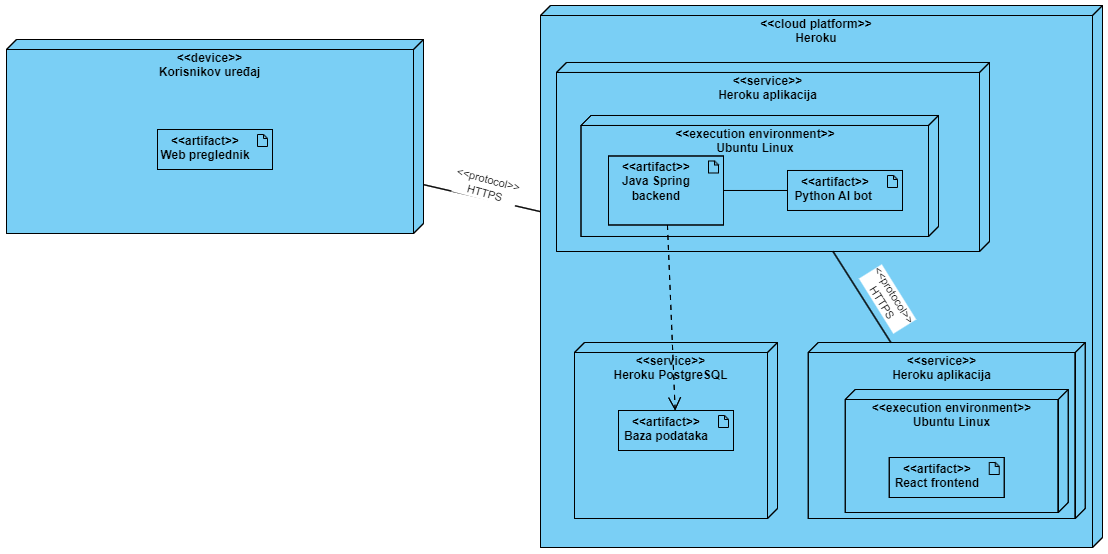
\includegraphics[width=1\linewidth]{slike/Dijagram razmjestaja.png}
             \caption{Dijagram razmještaja}
             \end{figure}
			\eject
		
		\section{Upute za puštanje u pogon}
		
		
U postavljanju i puštanju u pogon naše aplikacije ključnu ulogu igra Heroku CLI (Command Line Interface), moćan naredbeni alat koji pojednostavljuje interakciju s Heroku platformom izravno iz terminala. Instalirali smo Heroku CLI na lokalnom računalu kako bismo iskoristili njegove funkcionalnosti za upravljanje aplikacijama na Heroku platformi.

Naša integrirana strategija razvoja i puštanja u pogon koristi niz ključnih značajki Heroku platforme:

1. Automatsko puštanje u pogon s GitHub-a:
   - GitHub repozitorij povezan je s Heroku, omogućujući jednostavano automatsko puštanje u pogon naše aplikacije.
   - Svaka promjena na glavnoj grani GitHuba automatski pokreće puštanje u pogon na Heroku platformi.

2. Konfiguracijske Datoteke na Heroku:
   - Heroku nam omogućava preciznu konfiguraciju putem posebnih datoteka koje definiraju okruženje za našu aplikaciju.
   - Detaljno smo definirali parametre poput verzija jezika (Java, Python) i aktivnih profila za Spring.

3. Korištenje Financijske Potpore od Heroku:

   - Naša organizacija prima financijsku potporu od Heroku platforme, pružajući nam sredstva za korištenje resursa.


4. Baza Podataka na Heroku:
   - Integrirali smo Heroku Postgres "add-on" za potrebe baze podataka.
   - Heroku Postgres pruža siguran pristup bazama podataka putem pridruženih akreditiva.
   \begin{figure}[H]
       \centering
       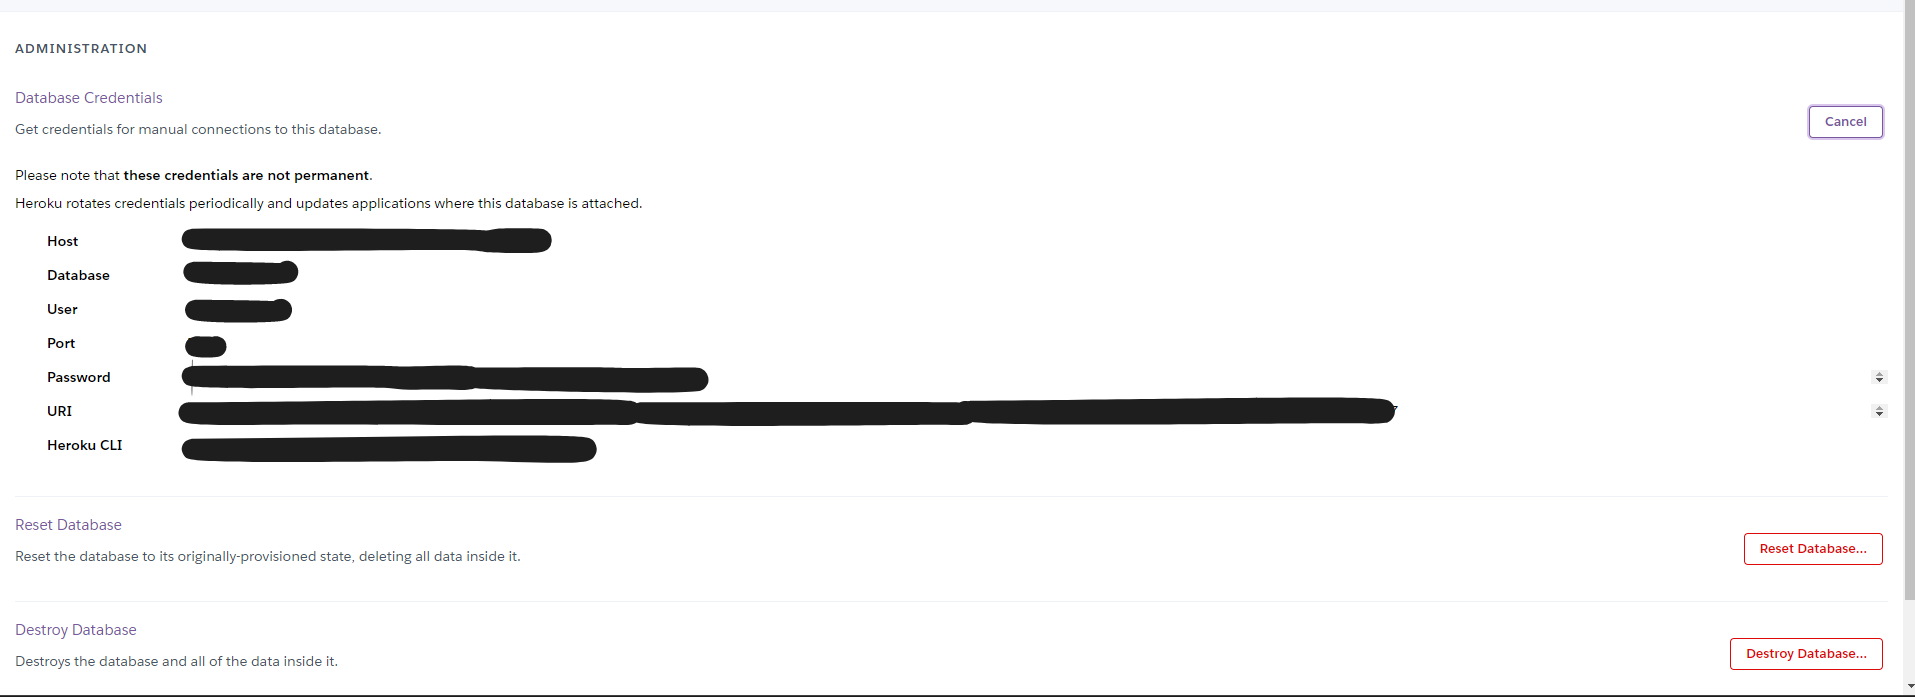
\includegraphics[width=1\linewidth]{slike/credentials.png}
       \caption{Akreditivi za našu aplikaciju}
       \label{fig:enter-label}
   \end{figure}

5. Dinamičko Okruženje s  dinamičkim kontejnerima:
   - Korištenjem dinamičkih kontejnera na Heroku stvaramo virtualno okruženje koje omogućuje izvršavanje i hostanje naše aplikacije.
   - Ime domene "medbay.life" registrirano je putem "Namecheap"-a, dok smo HTTPS certifikat dobili kroz Cloudflare za sigurnu komunikaciju.

6. Praćenje i evidentiranje:
   - Heroku pruža napredne alate za praćenje performansi, uključujući detaljne evidencije za svaki zahtjev poslan aplikaciji.
   - Metrike i analize omogućuju nam praćenje ponašanja aplikacije u stvarnom vremenu.
   \begin{figure}[H]
       \centering
       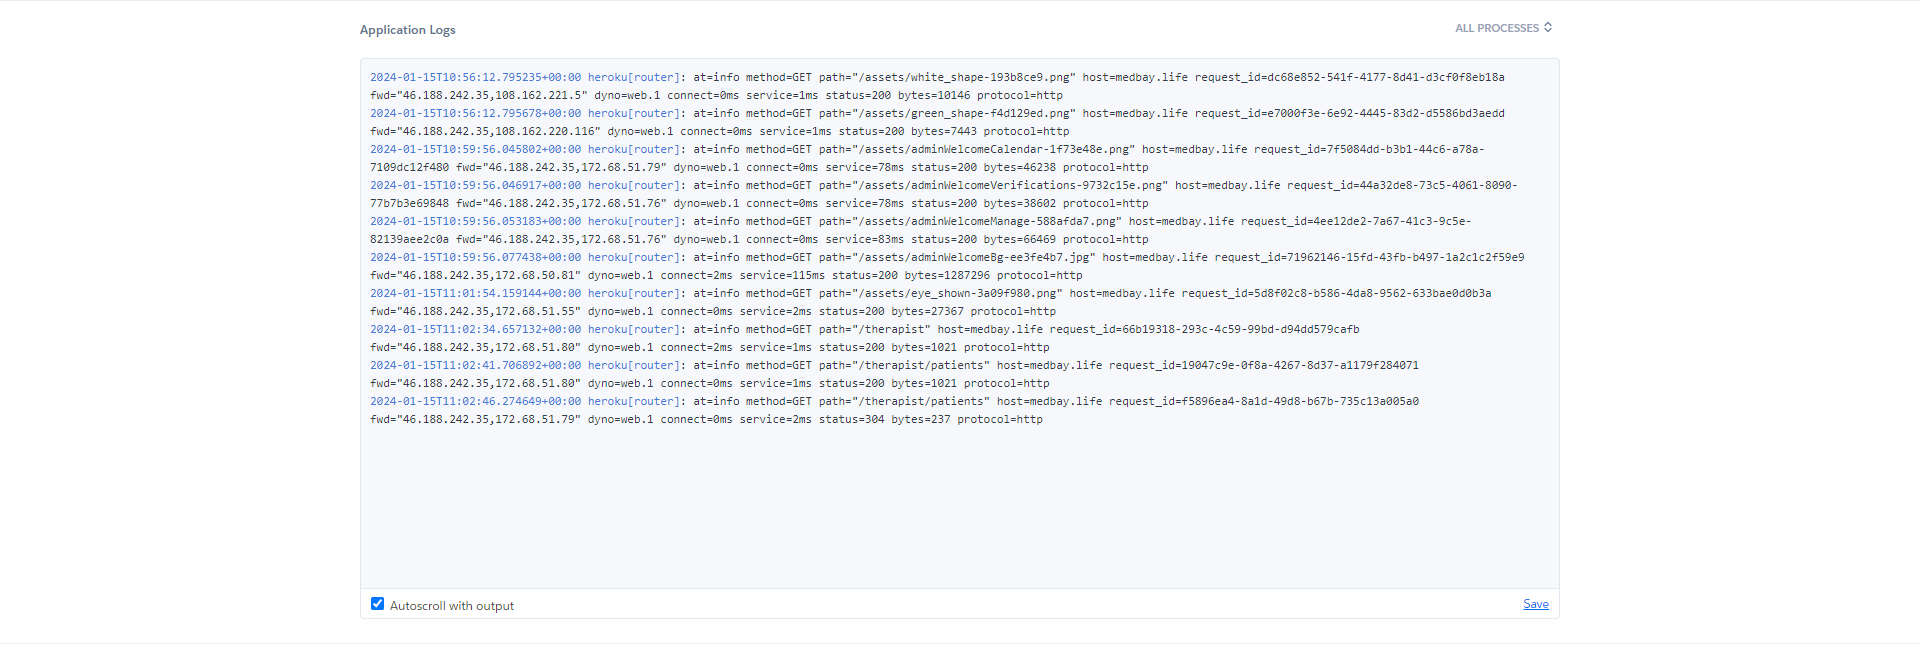
\includegraphics[width=1\linewidth]{slike/appLogs.png}
       \caption{Aplikacijsko evidentiranje}
       \label{fig:enter-label}
   \end{figure}


\begin{figure}[H]
    \centering
    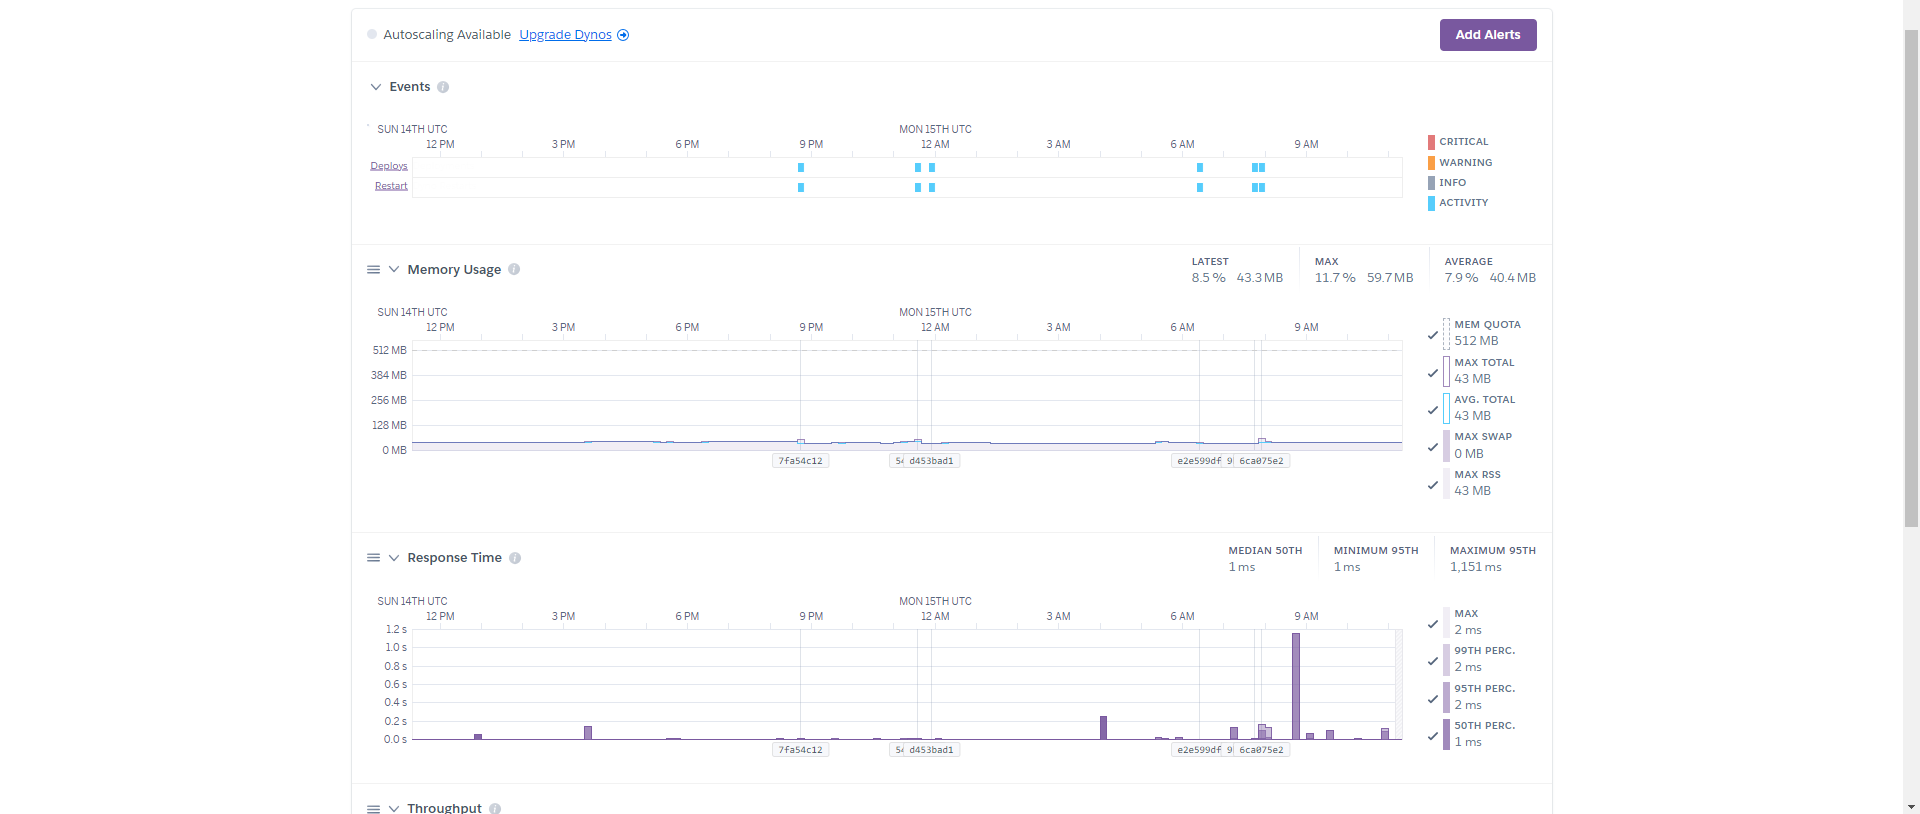
\includegraphics[width=1\linewidth]{slike/metrics.png}
    \caption{Metrika aplikacija}
    \label{fig:enter-label}
\end{figure}
7. Paketi za izgradnju:
   - Integrirali smo različite Pakete za izgradnju prilagođene jezicima koje koristimo (npr., Python, Java).
   - Automatski konfiguriraju okolinu i podržavaju različite jezične specifikacije.

Ovaj sveobuhvatan pristup omogućava nam efikasan ciklus razvoja i puštanja u pogon aplikacije. Kombinacijom GitHuba, Heroku platforme, i alata poput Heroku CLI-a, postižemo stabilan i automatski proces implementacije koji podržava dinamično okruženje naše aplikacije.


\textbf{Općenito o načinu korištenja Heroku CLI (Command Line Interface):}

1. Instalacija Heroku CLI:
   Heroku CLI smo instalirali na lokalnom računalu, omogućujući nam jednostavan pristup naredbama i funkcionalnostima koje pruža. Za instalaciju, slijedili smo upute dostupne na [službenoj Heroku stranici za instalaciju CLI-a](https://devcenter.heroku.com/articles/heroku-cli).

2. Povezivanje s Heroku Računom:
    Pomoću Heroku CLI-a uspostavili smo vezu s našim Heroku računom, omogućavajući autentikaciju i autorizaciju za izvršavanje različitih operacija. Ova faza je ključna za pristup resursima i upravljanje aplikacijom.

3. Korištenje CLI-a za puštanje u pogon aplikacije:
    Heroku CLI smo aktivno koristili za inicijalizaciju puštanje u pogon naših aplikacija. Naredbe poput `git push heroku main` omogućuju nam jednostavano i automatsko puštanje u pogon na Heroku platformu.

4. Upotreba CLI-a za Konfiguraciju Aplikacije:
    Heroku CLI pruža alate za konfiguraciju različitih aspekata aplikacije. Kroz naredbe poput `heroku config:set` postavljali smo i mijenjali okružne varijable te druge konfiguracijske postavke prema potrebama naše aplikacije.

5. Praćenje evidencija i Performansi:
    Za praćenje evidencija i performansi aplikacije koristili smo Heroku CLI. Naredbe poput `heroku logs` omogućuju nam pregled događaja u stvarnom vremenu, pružajući važne informacije o ponašanju aplikacije.

6. Dodatne Naredbe za Upravljanje Resursima:
    Heroku CLI pruža širok spektar dodatnih naredbi za upravljanje resursima. Skaliranje aplikacije, upravljanje "add-on"-ima i druge operacije mogu se jednostavno izvršiti putem ovog sučelja.

Heroku CLI je postao ključan alat u našem procesu razvoja i deploya. Omogućuje nam jednostavnu interakciju s Heroku platformom direktno iz terminala, čime poboljšavamo produktivnost i imamo veću kontrolu nad našim aplikacijama. 

